\title{Economic Time Series HW1}
\author{Daeyoung Lim}

\documentclass[answers]{exam}
\usepackage[left=3cm,right=3cm,top=3.5cm,bottom=2cm]{geometry}
\usepackage{amssymb,amsmath,amsfonts,amsthm}
\usepackage{mathtools}
\usepackage{graphicx}
\usepackage{kotex}
\usepackage[utf8]{inputenc}
\usepackage[T1]{fontenc}
\usepackage{lmodern}
% \usepackage{enumerate}
\usepackage{listings}
\usepackage{courier}
\usepackage{cancel}
\usepackage{array}
\usepackage{courier}
\usepackage{booktabs}
\usepackage{titlesec}
\usepackage[shortlabels]{enumitem}
\usepackage{setspace}
\usepackage{newtxtext}
\usepackage[lite,nofontinfo,zswash,straightbraces]{mtpro2}
\usepackage{empheq}
\usepackage{tikz}
\usepackage{listings}

% \usepackage[toc,page]{appendix}

\setlength{\heavyrulewidth}{1.5pt}
\setlength{\abovetopsep}{4pt}

\DeclarePairedDelimiter{\ceil}{\lceil}{\rceil}
\newcommand\encircle[1]{%
  \tikz[baseline=(X.base)] 
    \node (X) [draw, shape=circle, inner sep=0] {\strut #1};}
 
% Command "alignedbox{}{}" for a box within an align environment
% Source: http://www.latex-community.org/forum/viewtopic.php?f=46&t=8144
\newlength\dlf  % Define a new measure, dlf
\newcommand\alignedbox[2]{
% Argument #1 = before & if there were no box (lhs)
% Argument #2 = after & if there were no box (rhs)
&  % Alignment sign of the line
{
\settowidth\dlf{$\displaystyle #1$}  
    % The width of \dlf is the width of the lhs, with a displaystyle font
\addtolength\dlf{\fboxsep+\fboxrule}  
    % Add to it the distance to the box, and the width of the line of the box     ㅊ
\hspace{-\dlf}  
    % Move everything dlf units to the left, so that & #1 #2 is aligned under #1 & #2
\boxed{#1 #2}
    % Put a box around lhs and rhs
}
}
\setcounter{secnumdepth}{4}
\lstset{
         basicstyle=\footnotesize\ttfamily, % Standardschrift
         %numbers=left,               % Ort der Zeilennummern
         numberstyle=\tiny,          % Stil der Zeilennummern
         %stepnumber=2,               % Abstand zwischen den Zeilennummern
         numbersep=5pt,              % Abstand der Nummern zum Text
         tabsize=2,                  % Groesse von Tabs
         extendedchars=true,         %
         breaklines=true,            % Zeilen werden Umgebrochen
         keywordstyle=\color{red},
            frame=b,         
 %        keywordstyle=[1]\textbf,    % Stil der Keywords
 %        keywordstyle=[2]\textbf,    %
 %        keywordstyle=[3]\textbf,    %
 %        keywordstyle=[4]\textbf,   \sqrt{\sqrt{}} %
         stringstyle=\color{white}\ttfamily, % Farbe der String
         showspaces=false,           % Leerzeichen anzeigen ?
         showtabs=false,             % Tabs anzeigen ?
         xleftmargin=17pt,
         framexleftmargin=17pt,
         framexrightmargin=5pt,
         framexbottommargin=4pt,
         %backgroundcolor=\color{lightgray},
         showstringspaces=false      % Leerzeichen in Strings anzeigen ?        
 }
 \lstloadlanguages{% Check Dokumentation for further languages ...
         %[Visual]Basic
         %Pascal
         %C
         %C++
         %XML
         %HTML
         Java
 }
    %\DeclareCaptionFont{blue}{\color{blue}} 

\definecolor{myblue}{RGB}{72, 165, 226}
\definecolor{myorange}{RGB}{222, 141, 8}
\titleformat{\paragraph}
{\normalfont\normalsize\bfseries}{\theparagraph}{1em}{}
\titlespacing*{\paragraph}
{0pt}{3.25ex plus 1ex minus .2ex}{1.5ex plus .2ex}
\setlength{\heavyrulewidth}{1.5pt}
\setlength{\abovetopsep}{4pt}
\setlength{\parindent}{0mm}
\linespread{1.3}
\DeclareMathOperator{\sech}{sech}
\DeclareMathOperator{\csch}{csch}
\DeclareMathOperator*{\argmin}{\arg\!\min}
\DeclareMathOperator{\Tr}{Tr}

\newcommand{\bs}{\boldsymbol}
\newcommand{\opn}{\operatorname}
%%%%%%%%%%%%%%%%%%%%%%%%%%%%%%%%%%%%%%%%%%%%%%%%%%%%%%%
% % We use newtheorem to define theorem-like structures
% %
% % Here are some common ones. . .
%%%%%%%%%%%%%%%%%%%%%%%%%%%%%%%%%%%%%%%%%%%%%%%%%%%%%%%
% \newtheorem{theorem}{Theorem}
% \newtheorem{lemma}{Lemma}
% \newtheorem{proposition}{Proposition}
% \newtheorem{scolium}{Scolium}   %% And a not so common one.
% \newtheorem{definition}{Definition}
% \newenvironment{proof}{{\sc Proof:}}{~\hfill QED}
% \newenvironment{AMS}{}{}
% \newenvironment{keywords}{}{}
%%%%%%%%%%%%%%%%%%%%%%%%%%%%%%%%%%%%%%%%%%%%%%%%%%%%%%%
% %   The first thanks indicates your affiliation
% %
% %  Just the name here.
% %
% % Your mailing address goes at the end.
% %
% % \thanks is also how you indicate grant support
% %
%%%%%%%%%%%%%%%%%%%%%%%%%%%%%%%%%%%%%%%%%%%%%%%%%%%%%%%


\begin{document}
\setstretch{1.5} %줄간격 조정
\newpage
\firstpageheader{}{}{\bf\large Daeyoung Lim \\ Economic Time Series \\ Fall Semester, 2016}
\runningheader{Daeyoung Lim}{Economic Time Series}{Fall Semester, 2016}
\begin{questions}
  \question
  Replicate Figures 1,5,6 and 7 in the Matlab exercise. In doing so, make the following modifications to the figures.
  \begin{enumerate}[(1)]
    \item In figure 1, use ``plot'' instead of ``stairs'', and use a dotted line instead of a solid line.
    \item In figure 5, plot the data from Jan 2004 only and remove all grid lines.
    \item Put figures 6 and 7 on a common figure frame in $2\times 2$ format.
  \end{enumerate}
  \begin{solution}
    \begin{enumerate}[(1)]
      \item Figure 1
      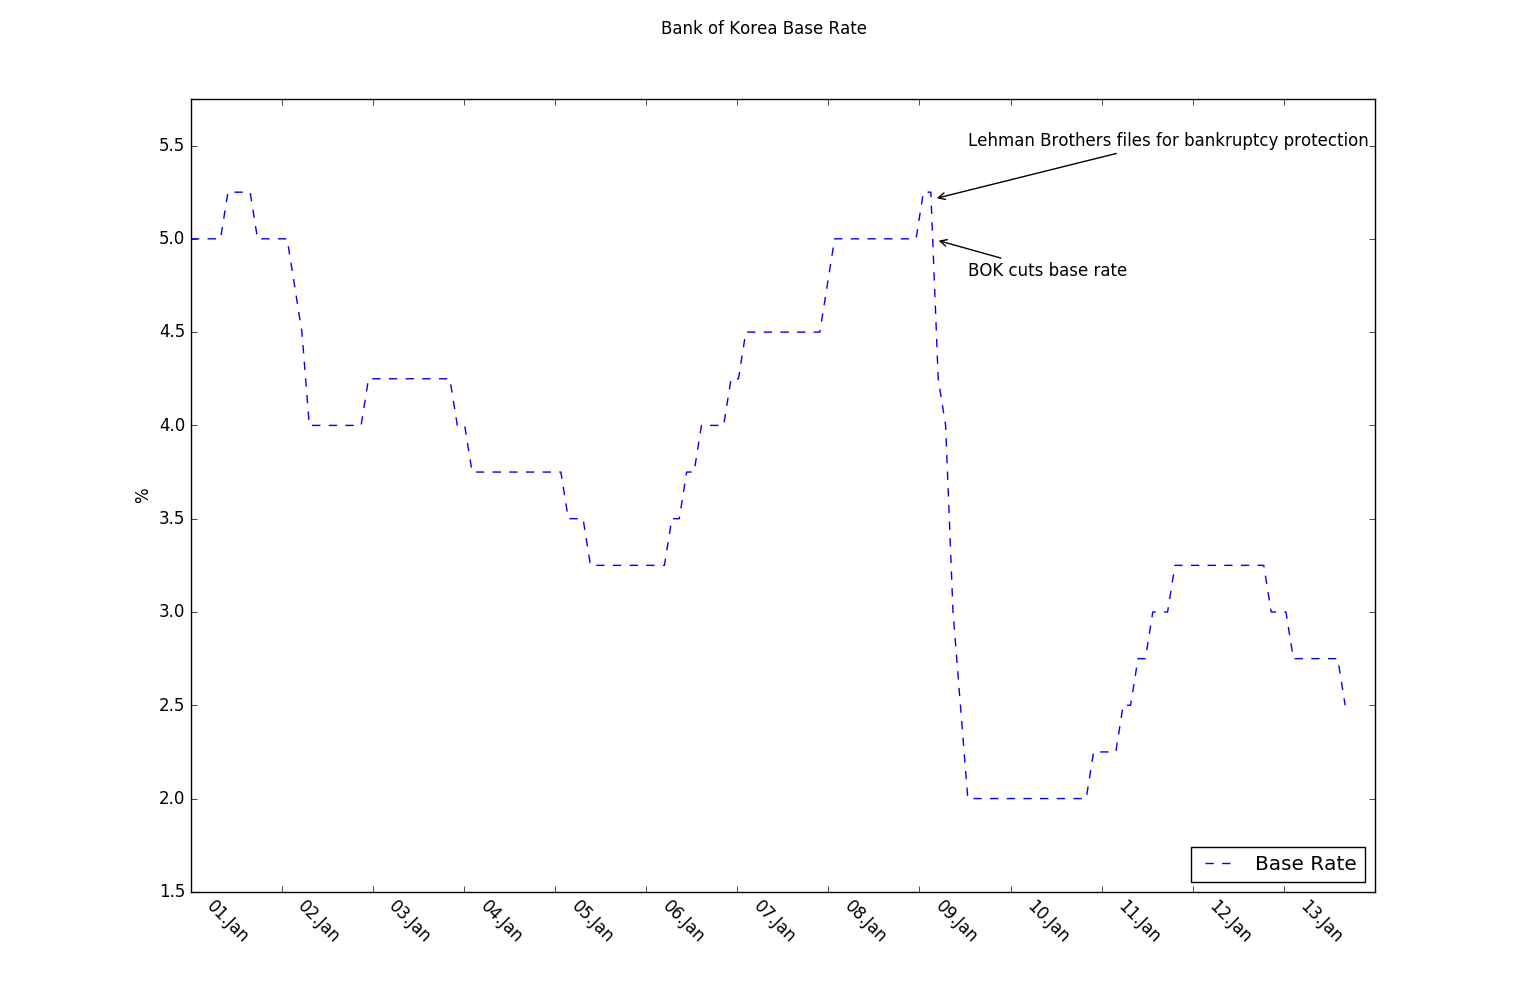
\includegraphics[scale=0.3]{figure_1.png}
      \item Figure 5
      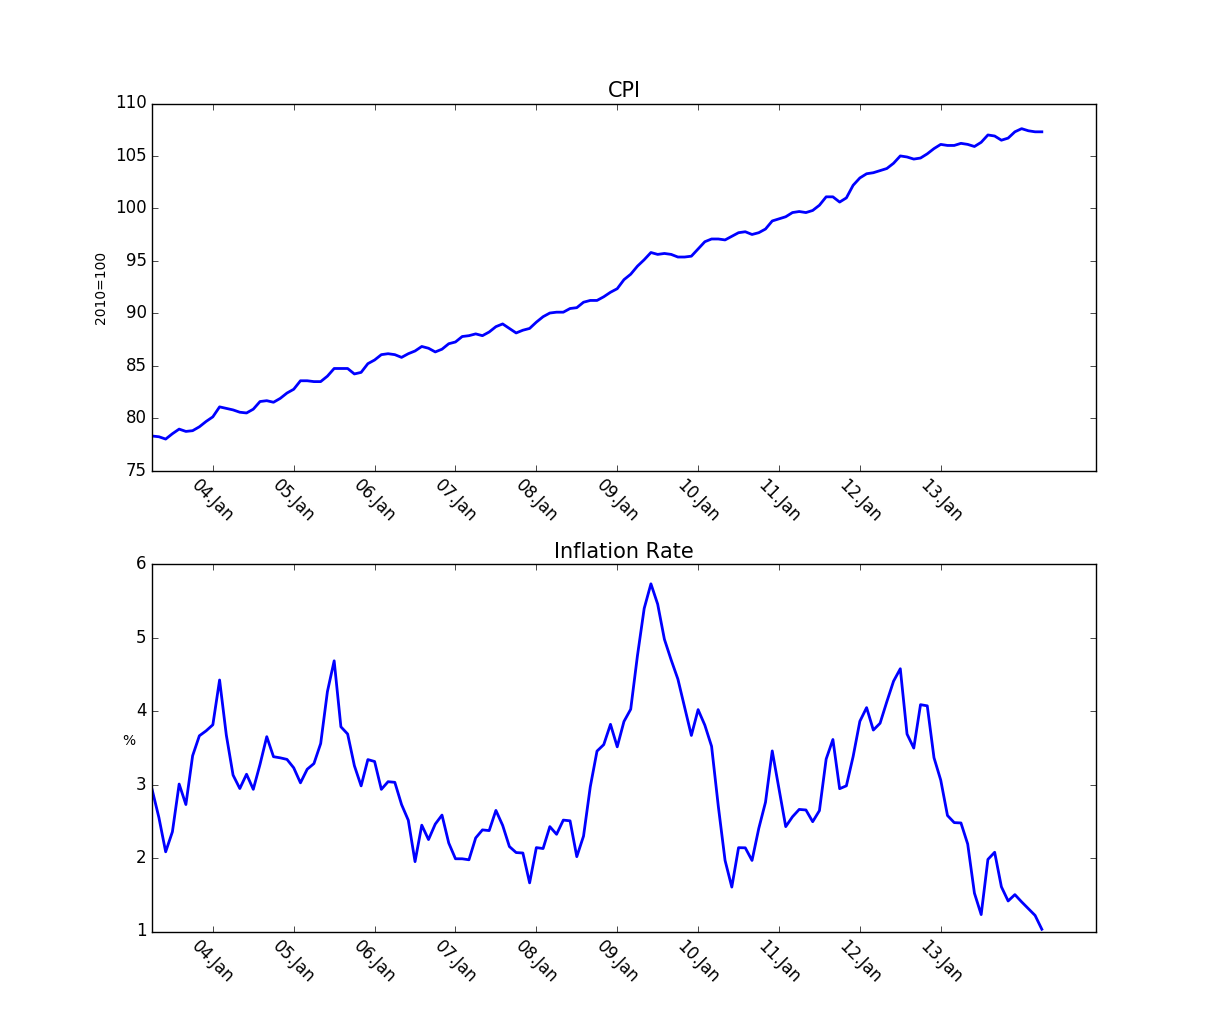
\includegraphics[scale=0.3]{figure_5.png}
      \item Figure 6 and 7
      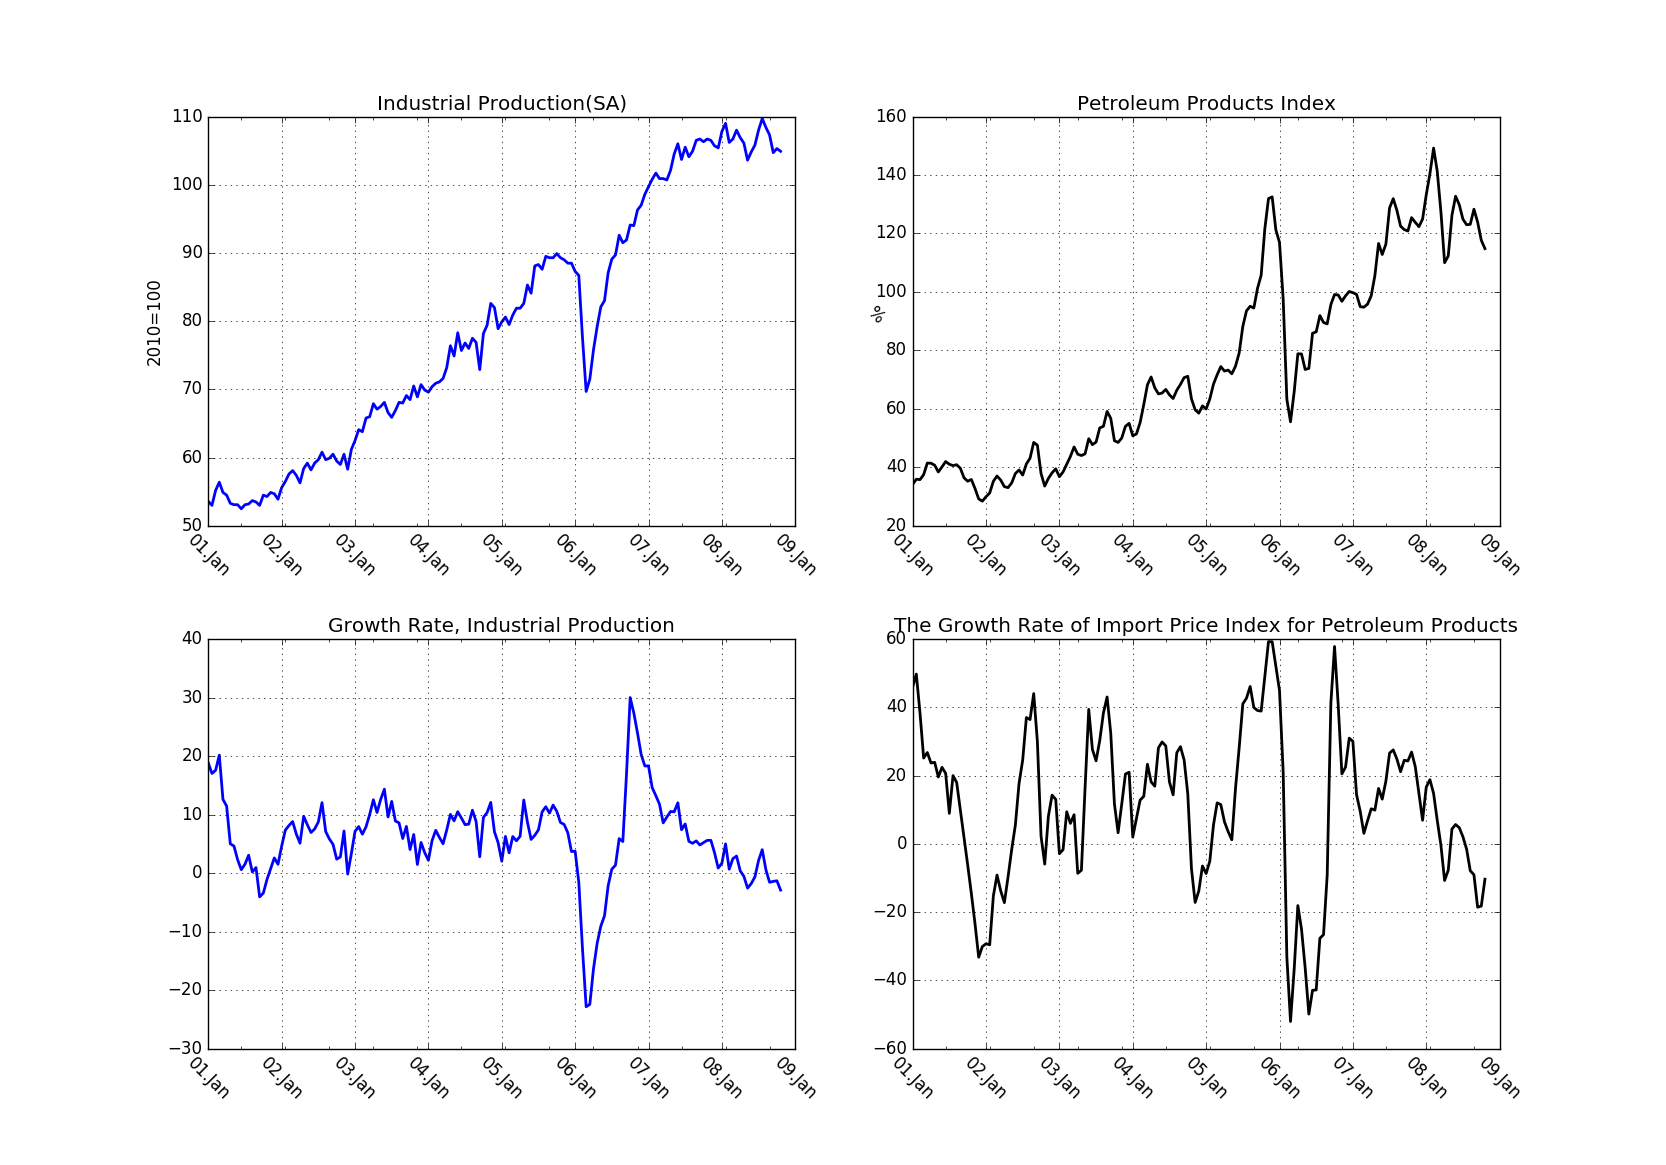
\includegraphics[scale=0.3]{figure_67.png}
    \end{enumerate}
  \end{solution}
  \question
  Suppose that the data are generated by the following model
  \begin{align}
    y &= X\beta+u\\
      &= X_{1}\beta_{1}+X_{2}\beta_{2}+u
  \end{align}
  where $X=\left[X_{1},X_{2}\right]$. Assume that $X$ is of full column rank, $T^{-1}X'X\xrightarrow{p}Q$, and $\beta_{2}\neq 0$. Denote the OLS estimate for (1) by $\what{\beta}_{1}$ and $\what{\beta}_{2}$. Suppose you estimate the regression
  \begin{equation}
    y=X_{1}\beta_{1}+e
  \end{equation}
  by OLS and denote the resulting estimate by $\what{b}_{1}$.
  \begin{enumerate}[a)]
    \item Show that $\what{b}_{1}$ is inconsistent for $\beta_{1}$, with assuming $\mathrm{E}\left(X_{1}'X_{2}^{}\right)\neq 0$.
    \item The inconsistency of $\what{b}_{1}$ is an example of the omitted variable bias. A natural estimate would then be based on an instrumental variable procedure. Show that the OLS estimate $\what{\beta}_{1}$ can indeed be given an IV interpretation.
  \end{enumerate}
  \begin{solution}
    \begin{enumerate}[a)]
      \item The omitted variable bias lingers even when the sample size grows large causing the estimators to be inconsistent. We can show this by simply plugging in the true model of $y$ to the estimator $\what{b}_{1}$.
      \begin{align}
        \what{b}_{1} &= \left(X_{1}'X_{1}\right)^{-1}X_{1}'y\\
        &= \left(X_{1}'X_{1}^{}\right)^{-1}X_{1}'\left(X_{1}\beta_{1}+X_{2}\beta_{2}+u\right)\\
        &= \beta_{1}+\left(X_{1}'X_{1}^{}\right)^{-1}X_{1}'X_{2}^{}\beta_{2}^{}+\left(X_{1}'X_{1}^{}\right)^{-1}X_{1}'u
      \end{align}
      The problem states that $\mathrm{E}\left(X_{1}'X_{2}^{}\right)\neq 0, \beta_{2}\neq 0$, preserving the second term. Note that the only \emph{random variable} in the above equation is $u$, converging in probability to zero as $T\to\infty$ where $T$ is the dimension of $y\, \left(T\times 1\right)$. Thus, there is no reason for the second term $\left(X_{1}'X_{1}^{}\right)^{-1}X_{1}'X_{2}^{}\beta_{2}^{}$ to disappear.
      \begin{equation}
        \what{b}_{1}\xrightarrow{p} \beta_{1}+\beta_{2}\left(X_{1}'X_{1}^{}\right)^{-1}X_{1}'X_{2}^{}
      \end{equation}
      \item $X_{2}$ is by assumption independent of the error term $u$. Therefore, using the method of moment, if we have $\mathrm{E}\left(x_{i2}u_{i}\right)=0$,
      \begin{equation}
        \dfrac{1}{T}\sum_{t=1}^{T}x_{i2}u_{i}=\dfrac{1}{T}X_{2}'u=\dfrac{1}{T}X_{2}'\left(y-X_{1}\beta_{1}\right).
      \end{equation}
      Solving with respect to $\beta_{1}$ yields
      \begin{equation}
        \what{\beta}_{1} = \left(X_{2}'X_{1}^{}\right)^{-1}X_{2}'y
      \end{equation}
      which is the IV estimate.
    \end{enumerate}
  \end{solution}
  \question
  Consider the linear regression model:
  \begin{align}
    y &= X\beta+u\\
    y,u &: T\times 1\\
    X &: T\times k\\
    \beta &: k\times 1
  \end{align}
  with the $q$ moment conditions $\mathrm{E}\left(z_{t}u_{t}\right)=0$. Let
  \begin{equation}
    J_{T}\left(\beta,W_{T}\right)=g_{T}\left(\beta\right)'W_{T}g_{T}\left(\beta\right)
  \end{equation}
  where $g_{T}\left(\beta\right)=T^{-1}\sum z_{t}\left(y_{t}-x_{t}'\beta\right)$ and $W_{T}$ is some weighting matrix. The GMM estimator for $\beta$ is obtained as the minimizer of $J_{T}\left(\beta,W_{T}\right)$.
  \begin{enumerate}[a)]
    \item How does your choice of $W_{T}$ affect the GMM estimator? Discuss the implications on the consistency, the asymptotic normality and efficiency.
    \item If the model is exactly identified $(k=q)$, explain why the choice of $W_{T}$ becomes irrelevant.
  \end{enumerate}
  \begin{solution}
    \begin{enumerate}[a)]
      \item 
      \begin{itemize}
        \item \emph{(Consistency)} Although the problem asked how the choice of $W_{T}$ affects the \emph{generalized method of moments} estimator, there are a few conditions that should hold in order for the estimator to be consistent.
        \begin{itemize}
          \item $g_{T}\left(\xi\right)$ should uniformaly converge in probability to the true moment $\mathrm{E}\left(z_{t}u_{t}\right)$ in $L_{2}$ space. That is, if we denote $g_{0}\left(\xi\right)=\mathrm{E}\left(z_{t}\left(y_{t}-x_{t}'\xi\right)\right)$,
          \begin{equation}
            \sup_{\xi\in\Xi}\left\|g_{T}\left(\xi\right)-g_{0}\left(\xi\right)\right\|_{2}\xrightarrow{p}0
          \end{equation}
          where $\beta$ is replaced with the notation $\xi$ for the time being and $\Xi$ is the whole parameter space.
          \item For all $\xi\in\Xi$ that are $\left\|\xi-\xi_{0}\right\|_{2}>\epsilon$, $J_{0}\left(\xi,W\right)-J_{0}\left(\xi_{0},W\right)>0$ where $J_{0}\left(\xi,W\right)=g_{0}\left(\xi\right)'Wg_{0}\left(\xi\right)$.
          \item $J_{T}\left(\xi\right)$ should be continuous.
        \end{itemize}
        With these assumptions, GMM will be consistent. Note that there is no requirement for $W_{T}$ except that it should be positive definite. In fact, we could relax this contraint so that $W_{T}$ is positive semi-definite but for the GMM to be consistent, $W_{T}\xrightarrow{p}W$ should still hold where $W$ is a positive definite constant matrix.
        \item \emph{(Asymptotic Normality)} Because we obtain GMM by minimizing $J_{T}\left(\xi,W_{T}\right)$, we need to specify the conditions that guarantee that there really is a minimum that we can reach. These are the following. Let us first define $\varphi\left(z_{t},\xi\right)\equiv z_{t}\left(y_{t}-x_{t}'\xi\right)$ where $z_{t},\varphi\left(z_{t},\xi\right)\in \mathbf{R}^{q}$.
        \begin{itemize}
          \item The parameter space $\Xi$ is compact.
          \item $J_{T}\left(\xi,W_{T}\right)$ is twice continuously differentiable.
          \item If we define the matrix $G=\mathrm{E}\left(\nabla_{\xi}g_{T}\left(\xi\right)\right)$, then $G'WG$ should be nonsingular, i.e., invertible, since the term is included in the expression of GMM.
          \item $\varphi\left(z_{t},\xi\right)\in L_{2}$. That is, $\varphi\left(z_{t},\xi\right)$ should have finite variance.
          \item $\mathrm{E}\left(\sup_{\xi\in\Xi}\left\|\nabla_{\xi}\varphi\left(z_{t},\xi\right)\right\|\right)<\infty$ so as to apply the uniform law of large numbers.
        \end{itemize}
        Again, there is no special requirement for the weight matrix $W_{T}$. However, we can talk about the efficiencies of the GMM estimator across different weight matrices. When we compare two matrices, we say matrix $A$ is bigger than $B$ if $A-B$ is positive semi-definite and we denote this relation by $A\succeq B$. If $A-B$ is strictly positive definite, we denote this by $A \succ B$.\par
        With this relation, we can compare the variances of two GMM estimators that only differ in their weight matrices. Let us define $\Omega\left(\xi_{0}\right)$ to be the covariance matrix $\mathrm{E}\left[\varphi\left(z_{t},\xi_{0}\right)\varphi\left(z_{t},\xi_{0}\right)'\right]$ with regard to the true parameter $\xi_{0}$. Then in terms of the asymptotic variance of the GMM estimator, setting $W=\Omega^{-1}$ yields the most efficient result, meaning the variance is the smallest. We can prove this by the following procedure.
        \begin{align}
          &\left(G'WG\right)^{-1}G'W\Omega WG\left(G'WG\right)^{-1}-\left(G'\Omega^{-1}G\right)^{-1} \\
          &= \left(G'WG\right)^{-1}\left(G'W\Omega WG-G'WG\left(G'\Omega^{-1}G\right)^{-1}G'WG\right)\left(G'WG\right)^{-1}\\
          &= \left(G'WG\right)^{-1}G'W\Omega^{1/2}\left(I-\Omega^{-1/2}G\left(G'\Omega^{-1}G\right)^{-1}G'\Omega^{-1/2}\right)\Omega^{1/2}WG\left(G'WG\right)^{-1} \succ 0
        \end{align}
        Therefore, $\Omega^{-1}$ will always be smaller than any weight matrix $W$ in the asymptotic sense.
        % \item \emph{(Consistency)} We have since the beginning only required $W_{T}$ to be positive definite, which will in effect hold the optimization landscape to be convex and thus optimizable. However, relaxing the constraint to positive \emph{semi}-definiteness will leave the posibility of $J_{T}\left(\what{\beta}^{\text{GMM}},W_{T}\right)=0$ wide open, violating the sample moment conditions. However, as long as $W_{T}$ converges to a positive definite symmetric matrix $W$ as $T\to\infty$, the GMM will still be consistent.
        % \item \emph{(Asymptotic Normality)} If the estimator is consistent($W_{T}\xrightarrow{p}W$)---which requires that $W_{T}$ is asymptotically positive definite---alongside some conditions regarding the \emph{Central Limit Theorem}, GMM will converge in distribution to a normal random variable. 
      \end{itemize}
      \item If the model is exactly identified, i.e., $k=q$, then the first-order condition of the objective function
      \begin{equation}
        X'ZW_{T}Z'\left(y-X\xi\right)=0
      \end{equation}
      whose $X'Z$ term is a square matrix. Thus, if we premultiply both sides by $W_{T}^{-1}\left(X'Z\right)^{-1}$, the solution gets reduced to the IV estimator. It indicates that the estimator can be chosen independently of the weight matrix $W_{T}$ if the model is fully identified.
    \end{enumerate}
  \end{solution}
  \question
  Let $y_{t}\overset{\text{iid}}{\sim}\mathrm{Exp}\left(\theta\right)$ for $t=1,\ldots,T$.
  \begin{enumerate}[a)]
    \item Derive the score function, Hessian function and information matrix, using the exponential density.
    \item Derive the MLE for $\theta$. Sketch the proof that the MLE is asymptotically normal. Be specific with the asymptotic variance.
  \end{enumerate}
  \begin{solution}
    \begin{enumerate}[a)]
      \item The likelihood function of $y_{1},\ldots,y_{T}$,
      \begin{equation}
        L\left(\theta\,\middle|\,y_{1}\ldots,y_{T}\right) = \theta^{T}\exp\left(-\theta\sum_{t=1}^{T}y_{t}\right).
      \end{equation}
      Taking the logarithm yields
      \begin{equation}
        \ell\left(\theta\,\middle|\,y_{1},\ldots,y_{T}\right) = T\log\theta-\theta\sum_{t=1}^{T}y_{t}.
      \end{equation}
      By definition of the score function is the first derivative of the log-likelihood.
      \begin{equation}
        \dfrac{d\ell}{d\theta} = \dfrac{T}{\theta}-\sum_{t=1}^{T}y_{t}.
      \end{equation}
      The Hessian gets reduced to the second derivative for a univariate function.
      \begin{equation}
        \dfrac{d^{2}\ell}{d\theta^{2}} = -\dfrac{T}{\theta^{2}}-\sum_{t=1}^{T}y_{t}.
      \end{equation}
      To get the Fisher information,
      \begin{align}
        \mathcal{I}_{T}\left(\theta\right) &= \dfrac{1}{T}\mathrm{E}\left(\dfrac{T}{\theta^{2}}+\sum_{t=1}^{T}y_{t}\right)\\
        &= \dfrac{1}{\theta^{2}}+\dfrac{1}{T}\sum_{t=1}^{T}\mathrm{E}\left(y_{t}\right)\\
        &= \dfrac{1}{\theta^{2}}+\dfrac{1}{\theta}
      \end{align}
      \item We have obtained the first and second derivatives of the log-likelihood already. Recall:
      \begin{align}
        \dfrac{d\ell}{d\theta} &= \dfrac{T}{\theta}-\sum_{t=1}^{T}y_{t}\\
        \dfrac{d^{2}\ell}{d\theta^{2}} &= -\dfrac{T}{\theta^{2}}-\sum_{t=1}^{T}y_{t}
      \end{align}
      Using the first-order condition, the MLE comes with a closed-form expression.
      \begin{equation}
        \what{\theta}^{\text{MLE}} = \left.T\middle/\left(\sum_{t=1}^{T}y_{t}\right)\right.
      \end{equation}
      The second-order condition validates that the estimator is actually a maximum since
      \begin{equation}
        \dfrac{d^{2}\ell}{d\theta^{2}} < 0.
      \end{equation}
      Now, even as rough a proof as what we will shortly give here takes at least 2 steps: the consistency of MLE and the asymptotic normality of MLE.
      \begin{itemize}
        \item \emph{(Consistency)} Recall that we take the product of every single PDF of $y_{t}$ through $t=1,\ldots,T$ to compute the likelihood function, which also means taking the logarithm will convert the product into summation.
        \begin{equation}
          \ell\left(\theta\,\middle|\,y_{1},\ldots,y_{T}\right) = \sum_{t=1}^{T}\ell\left(\theta\,\middle|\,y_{t}\right)
        \end{equation}
        By the strong law of large numbers, we get the following relation:
        \begin{equation}\label{eq:1}
          \dfrac{1}{T}\sum_{t=1}^{T}\ell\left(\theta\,\middle|\,y_{t}\right)\xrightarrow{a.s.}\mathrm{E}_{\theta_{\circ}}\ell\left(\theta\,\middle|\,y_{1}\right)
        \end{equation}
        for some unknown true parameter value $\theta_{\circ}$. We can then show that the expected log-likelihood function w.r.t. the true parameter is always greater than that of an arbitrary parameter $\theta$ by \emph{Kullback-Leibler divergence}. The KL divergence is defined as follows.
        \begin{align}
          \mathrm{KL}\left(f(y_{1}\,|\,\theta_{\circ})\,\middle\|\,f(y_{1}\,|\,\theta)\right) &= \mathrm{E}_{\theta_{\circ}}\left[\log \dfrac{f(y_{1}\,|\,\theta_{\circ})}{f(y_{1}\,|\,\theta)} \right]\\
          &= -\int \log \dfrac{f(y_{1}\,|\,\theta)}{f(y_{1}\,|\,\theta_{\circ})}\; f(y_{1}\,|\,\theta_{\circ})\,dy_{1}
        \end{align}
        By \emph{Jensen's inequality},
        \begin{equation}
          \underbrace{-\log\int \dfrac{f(y_{1}\,|\,\theta)}{\cancel{f(y_{1}\,|\,\theta_{\circ})}}\; \cancel{f(y_{1}\,|\,\theta_{\circ})}\,dy_{1}}_{=0} \leq \underbrace{-\int \log \dfrac{f(y_{1}\,|\,\theta)}{f(y_{1}\,|\,\theta_{\circ})}\; f(y_{1}\,|\,\theta_{\circ})\,dy_{1}}_{=\mathrm{KL}\left(f(y_{1}\,|\,\theta_{\circ})\,\middle\|\,f(y_{1}\,|\,\theta)\right) }.
        \end{equation}
        Therefore, it always follows that the KL divergence is nonnegative. In fact, it is strictly positive if $f(y_{1}\,|\,\theta)\neq f(y_{1}\,|\,\theta_{\circ})$.
      This indicates that
      \begin{equation}
        \theta_{\circ} = \sup_{\theta\in\Omega}\mathrm{E}_{\theta_{\circ}}\ell\left(\theta\,\middle|\,y_{1}\right).
      \end{equation}
      Recall the following:
      \begin{equation}
        \what{\theta}^{\text{MLE}} = \sup_{\theta\in\Omega}\dfrac{1}{T}\sum_{t=1}^{T}\ell\left(\theta\,\middle|\,y_{i}\right).
      \end{equation}
      Therefore by \ref{eq:1}, $\what{\theta}^{\text{MLE}}\xrightarrow{p} \theta_{\circ}$ for a finite parameter space $\Omega$. We can also prove this for a compact parameter space by starting from the lemma that
      \begin{equation}
        \dfrac{1}{T}\sum_{t=1}^{T}\ell\left(\theta\,|\,y_{t}\right)\xrightarrow{\text{uniformly convergent}} \int \ell\left(\theta\,|\,y_{1}\right)f(y_{1}\,|\,\theta_{0})\,dy_{1}\quad \left(=\mathrm{E}_{\theta_{0}}\ell\left(\theta\,|\,y_{1}\right)\right)
      \end{equation}
      which is equivalent to
      \begin{equation}\label{almostSure}
        \mathrm{Pr}\left(\sup_{\theta\in\Omega}\left|\dfrac{1}{T}\sum_{t=1}^{T}\ell\left(\theta\,|\,y_{t}\right)-\mathrm{E}_{\theta_{0}}\ell\left(\theta\,|\,y_{1}\right)\right|>\epsilon\right)\xrightarrow{a.s.} 0,\quad \forall \epsilon >0.
      \end{equation}
      Pointwise convergence is not enough with infinite parameter spaces because the convergence at one parameter of the log-likelihood function as a function of $y_{1:T}$ does not guarantee that the log-likelihood function with another set of $y_{1:T}$ generated with a different parameter value is also close to the true expected log-likelihood. Thus, the convergence at one parameter value does not generalize and we end up having to prove for infinitely many parameters which is not possible. Uniform convergence addresses such a problem all at once. Anyway, the proof for the consistency of MLE ends here.
      \item \emph{(Asymptotic Normality)} We approximate the score function with its first-order Taylor expansion around the true parameter $\theta_{\circ}$ and apply the mean value theorem.
      \begin{equation}
        \dfrac{d\ell}{d\theta} \approx \left.\dfrac{d\ell}{d\theta}\right|_{\theta=\theta_{\circ}}+\left.\dfrac{d^{2}\ell}{d\theta^{2}}\right|_{\theta=\overline{\theta}}\left(\theta-\theta_{\circ}\right)
      \end{equation}
      where $\overline{\theta}$ lies somewhere between $\theta$ and $\theta_{\circ}$. Since MLE is the value which sets the first derivative to zero, we can think of the following identity.
      \begin{equation}
        \left.\dfrac{d\ell}{d\theta}\right|_{\theta=\theta_{\circ}}+\left.\dfrac{d^{2}\ell}{d\theta^{2}}\right|_{\theta=\overline{\theta}}\left(\what{\theta}^{\text{MLE}}-\theta_{\circ}\right)=0
      \end{equation}
      This, in turn, translates to the following relationship.
      \begin{equation}\label{asympNorm}
        \what{\theta}^{\text{MLE}}-\theta_{\circ} =-\left.\left(\left.\dfrac{d\ell}{d\theta}\right|_{\theta=\theta_{\circ}}\right)\middle/\left(\left.\dfrac{d^{2}\ell}{d\theta^{2}}\right|_{\theta=\overline{\theta}}\right)\right.
      \end{equation}
      with $\overline{\theta} = s\what{\theta}^{\text{MLE}}+\left(1-s\right)\theta_{\circ},\; s\in\left[0,1\right]$. Let's slowly examine the RHS of \ref{asympNorm}. First, the numerator can be expressed as a summation of the log-likelihood of a single observation.
      \begin{equation}
        \left.\dfrac{d\ell\left(\theta\,|\,y_{1:T}\right)}{d\theta}\right|_{\theta=\theta_{\circ}} = \sum_{t=1}^{T}\left.\dfrac{d\ell\left(\theta\,|\,y_{t}\right)}{d\theta}\right|_{\theta=\theta_{\circ}}
      \end{equation}
      By the \emph{Central Limit Theorem},
      \begin{align}\label{CLT}
        \mathrm{E}\left(\left.\dfrac{d\ell\left(\theta\,|\,y_{1}\right)}{d\theta}\right|_{\theta=\theta_{\circ}}\right) &= 0\\
        \mathrm{Var}\left(\left.\dfrac{d\ell\left(\theta\,|\,y_{1}\right)}{d\theta}\right|_{\theta=\theta_{\circ}}\right) &= T\mathcal{I}_{1}\left(\theta\right)\\
        \left.\dfrac{d\ell\left(\theta\,|\,y_{1:T}\right)}{d\theta}\right|_{\theta=\theta_{\circ}} \xrightarrow{d} \mathcal{N}\left(0,T\mathcal{I}_{1}\left(\theta_{\circ}\right)\right)
      \end{align}
      where $\mathcal{I}_{1}$ is the Fisher information for a single observation $y_{1}$. The calculations for the expectation and the variance are given in the end. Now the denominator behaves like the following which makes use of the weak law of large numbers. (As is the case with consistency, if the parameter space is infinite, we need the uniform law of large numbers since we cannot say that the convergence around one parameter value does not guarantee the convergence around another. Anyway, we skip this part.)
      \begin{equation}\label{WLLN}
        \left.\dfrac{d^{2}\ell\left(\theta\,\middle|\,y_{1:T}\right)}{d\theta^{2}}\right|_{\theta=\overline{\theta}}=\sum_{t=1}^{T}\left.\dfrac{d^{2}\ell\left(\theta\,\middle|\,y_{t}\right)}{d\theta^{2}}\right|_{\theta=\overline{\theta}} \xrightarrow{p} T\mathrm{E}\left(\left.\dfrac{d^{2}\ell\left(\theta\,\middle|\,y_{1}\right)}{d\theta^{2}}\right|_{\theta=\overline{\theta}} \right) =-T\mathcal{I}_{1}\left(\overline{\theta}\right)
      \end{equation}
      With \ref{CLT}, \ref{WLLN}, and the \emph{Slutsky's theorem}, we can conclude that \ref{asympNorm} converges in distribution to a normal distribution.
      \begin{equation}
        -\left.\left(\left.\dfrac{d\ell}{d\theta}\right|_{\theta=\theta_{\circ}}\right)\middle/\left(\left.\dfrac{d^{2}\ell}{d\theta^{2}}\right|_{\theta=\overline{\theta}}\right)\right. \xrightarrow{d} \mathcal{N}\left(0,\dfrac{T\mathcal{I}_{1}\left(\theta_{\circ}\right)}{\left(T\mathcal{I}_{1}\left(\overline{\theta}\right)\right)^{2}}=\dfrac{\mathcal{I}_{T}\left(\theta_{\circ}\right)}{\left(\mathcal{I}_{T}\left(\overline{\theta}\right)\right)^{2}}\right)
      \end{equation}
      Finally, we know that $\overline{\theta}\in \left[\what{\theta}^{\text{MLE}},\theta_{\circ}\right]$ if $\what{\theta}^{\text{MLE}} < \theta_{\circ}$ or $\overline{\theta}\in \left[\theta_{\circ},\what{\theta}^{\text{MLE}}\right]$ if $\what{\theta}^{\text{MLE}} \geq \theta_{\circ}$. As $T\to\infty$, $\what{\theta}^{\text{MLE}}\xrightarrow{p}\theta_{\circ}$ which also means $\overline{\theta}\xrightarrow{p}\theta_{\circ}$. Thus,
      \begin{equation}
        \what{\theta}^{\text{MLE}} \xrightarrow{d} \mathcal{N}\left(\theta_{\circ},\left(\mathcal{I}_{T}\left(\theta_{\circ}\right)\right)^{-1}\right)
      \end{equation}
      \end{itemize}
    \end{enumerate}
    There are 3 different ways to compute the Fisher information and all three are equivalent under regularity conditions. The three are
    \begin{align}
      \mathcal{I}\left(\theta\right) &= \mathrm{E}\left(\left(\dfrac{d\ell}{d\theta}\right)^{2}\right)\\
      &= -\mathrm{E}\left(\dfrac{d^{2}\ell}{d\theta^{2}}\right)\\
      &= \mathrm{Var}\left(\dfrac{d\ell}{d\theta}\right)
    \end{align}
  \end{solution}
  \end{questions}
  \appendix
  \section{Code for Figure 1}
  \begin{lstlisting}[language=Python]
    import numpy as np
    import matplotlib.pyplot as plt
    import matplotlib.text as txt
    import types

    def rate(y,lag):
      T = len(y)
      g = (np.log(y[lag:T])-np.log(y[0:(T-lag)]))*100.
      return g

    data = np.loadtxt('/Users/daeyounglim/Downloads/data.txt',skiprows=1)
    date = data[:,0]
    base = data[:,1]
    cpi  = data[:,2]
    inf  = rate(cpi,12)
    imp_price = data[:,3]
    dimp_price = rate(imp_price,12)
    ip = data[:,5]
    dip = rate(ip,12)

    labels = ['01.Jan','02.Jan','03.Jan','04.Jan','05.Jan','06.Jan','07.Jan','08.Jan','09.Jan','10.Jan','11.Jan','12.Jan','13.Jan']
    fig,ax = plt.subplots()
    fig.suptitle('Bank of Korea Base Rate')
    line, = ax.plot(base[12:],label='Base Rate',linestyle='--')
    plt.ylim([1.5,np.max(base[12:])+.5])
    #ax = plt.axes()
    plt.xticks(list(range(9,165,12)),labels)
    # start,end = ax.get_xlim()
    # ax.xaxis.set_ticks(np.arange(start,end,(end-start)/13.))
    ax.set_xticklabels(labels,rotation=-45)
    ax.annotate('Lehman Brothers files for bankruptcy protection',xy=(100.441,5.21404),xytext=(105,5.5),
                arrowprops=dict(facecolor='black',arrowstyle='->'))
    ax.annotate('BOK cuts base rate',xy=(100.688,4.99432),xytext=(105,4.8),
                arrowprops=dict(facecolor='black',arrowstyle='->'))
    legend = plt.legend(handles=[line],loc=4)

    plt.ylabel('%')
    for lab in ax.xaxis.get_majorticklabels():
      lab.customShiftValue = 5.
      lab.set_x = types.MethodType(lambda self,x:  txt.Text.set_x(self, x+self.customShiftValue), 
                                        lab)
    plt.show()
  \end{lstlisting}
  \section{Code for Figure 5}
  \begin{lstlisting}
    import numpy as np
    import matplotlib.pyplot as plt
    import matplotlib.text as txt
    import types

    def rate(y,lag):
      T = len(y)
      g = (np.log(y[lag:T])-np.log(y[0:(T-lag)]))*100.
      return g

    data = np.loadtxt('/Users/daeyounglim/Downloads/data.txt',skiprows=1)
    date = data[:,0]
    base = data[:,1]
    cpi  = data[:,2]
    inf  = rate(cpi,12)
    imp_price = data[:,3]
    dimp_price = rate(imp_price,12)
    ip = data[:,5]
    dip = rate(ip,12)


    # labels = ['01.Jan','02.Jan','03.Jan','04.Jan','05.Jan','06.Jan','07.Jan','08.Jan','09.Jan','10.Jan','11.Jan','12.Jan','13.Jan']
    labels = ['04.Jan','05.Jan','06.Jan','07.Jan','08.Jan','09.Jan','10.Jan','11.Jan','12.Jan','13.Jan']
    fig,(ax1,ax2) = plt.subplots(2,1,sharex=False)
    # line, = ax1.plot(cpi[12:],linewidth=2.)
    line, = ax1.plot(cpi[36:],linewidth=2.)
    line2, = ax2.plot(inf[24:],linewidth=2.)
    ax1.xaxis.set_ticks(list(range(9,129,12)))
    ax1.set_xticklabels(labels,rotation=-45)
    ax2.xaxis.set_ticks(list(range(9,129,12)))
    ax2.set_xticklabels(labels,rotation=-45)
    ax1.set_ylabel('2010=100',fontsize=10)
    ax2.set_ylabel('%',fontsize=10,rotation=0)
    ax1.set_title('CPI',fontsize=15)
    ax2.set_title('Inflation Rate',fontsize=15)
    plt.show()
  \end{lstlisting}
  \section{Code for Figure 6 and 7}
  \begin{lstlisting}
    import numpy as np
    import matplotlib.pyplot as plt
    import matplotlib.text as txt
    import types

    def rate(y,lag):
      T = len(y)
      g = (np.log(y[lag:T])-np.log(y[0:(T-lag)]))*100.
      return g

    data = np.loadtxt('/Users/daeyounglim/Downloads/data.txt',skiprows=1)
    date = data[:,0]
    base = data[:,1]
    cpi  = data[:,2]
    inf  = rate(cpi,12)
    imp_price = data[:,3]
    dimp_price = rate(imp_price,12)
    ip = data[:,5]
    dip = rate(ip,12)

    labels = ['01.Jan','02.Jan','03.Jan','04.Jan','05.Jan','06.Jan','07.Jan','08.Jan','09.Jan','10.Jan','11.Jan','12.Jan','13.Jan']
    plt.figure(figsize=(2,2))
    ax1 = plt.subplot(221)
    ax2 = plt.subplot(222)
    ax3 = plt.subplot(223)
    ax4 = plt.subplot(224)
    # fig,(ax1,ax2,ax3,ax4) = plt.subplots(2,2,sharex=False)
    line1, = ax1.plot(ip[12:],'b',linewidth=2.)
    line2, = ax3.plot(dip,'b',linewidth=2.)
    line3, = ax2.plot(imp_price[12:],'k',linewidth=2.)
    line4, = ax4.plot(dimp_price,'k',linewidth=2.)
    ax1.set_title('Industrial Production(SA)')
    ax2.set_title('Petroleum Products Index')
    ax3.set_title('Growth Rate, Industrial Production')
    ax4.set_title('The Growth Rate of Import Price Index for Petroleum Products')
    ax1.set_ylabel('2010=100')
    ax2.set_ylabel('%',rotation=-45)
    ax1.set_xticks(list(range(9,165,12)),labels)
    ax1.set_xticklabels(labels,rotation=-45)
    ax1.grid(True)
    ax2.set_xticks(list(range(9,165,12)),labels)
    ax2.set_xticklabels(labels,rotation=-45)
    ax2.grid(True)
    ax3.set_xticks(list(range(9,165,12)),labels)
    ax3.set_xticklabels(labels,rotation=-45)
    ax3.grid(True)
    ax4.set_xticks(list(range(9,165,12)),labels)
    ax4.set_xticklabels(labels,rotation=-45)
    ax4.grid(True)

    plt.show()
  \end{lstlisting}
\end{document}
